\documentclass[12 pt, a4paper]{article}
\usepackage[utf8]{inputenc}
\usepackage[english, russian]{babel}
 \usepackage{graphicx}

\title{Алгоритм Форчуна}
\author{Быкова Анна Вадимовна}
\date{Октябрь 2022}

\begin{document}

\maketitle

\section{Введение}
\subsection{Суть и назначение}
Алгоритм Форчуна – это алгоритм заметающей прямой для генерации диаграммы Вороного из набора точек на плоскости за время O(n log n) с использованием памяти O(n).
\subsection{Авторство}
Данный алгоритм был опубликован Стивеном Форчуном в 1986 году в Нью Джерси. Статья носит название «A Sweepline Algorithm for Voronoi Diagrams» 
\subsection{История развития}
Алгоритм увидел свет в 1986 году.
\subsection{Перспектива Использования}
Алгоритм используется для построения диаграммы Вороного, которая в свою очередь имеет широкий спектр применения. 
Она используется в разнообразном геолокационном софте, особенно те, которые показывают распределение чего-либо. Так же применим и в архитектуре, дизайне, поскольку образует красивые причудливые формы. 
\newpage
\section{Описание метода}
\subsection{Формальное}
Основная идея алгоритма — это так называемая заметающая прямая (ЗП) (sweep line). Есть n сайтов (точек на плоскости). Есть заметающая прямая, которая двигается (например) «сверху вниз», то есть от сайта с наибольшей ординатой к сайту с меньшей (от события к событию, если быть точным). Сразу стоит отметить, что влияние на построение диаграммы оказывают только те сайты, которые находятся выше или на заметающей прямой.
Когда ЗП попадает на очередной сайт (происходит событие точки (point event)), создаётся новая парабола (arch), фокусом которой является данный сайт, а директрисой — заметающая прямая. Эта парабола делит плоскость на две части — «внутренняя» область параболы соответствует точкам, которые сейчас ближе к сайту, а «внешняя» область — точкам, которые ближе к sweep line, ну а точки, лежащие на параболе — равноудалены от сайта и ЗП. Парабола будет меняться в зависимости от положения ЗП к сайту — чем дальше ЗП уходит от сайта вниз, тем больше расширяется парабола, однако в самом начале она вообще является отрезком («направленным» вверх).
Далее парабола расширяется, у неё появляются две контрольные точки (break points) — точки её пересечения с остальными параболами («береговой линией»). В «береговой линии» мы храним дуги парабол от одной точки пересечения их друг с другом до другой, так и получается beach line. По сути, в этом алгоритме мы моделируем движение этой «береговой линии». потому как эти самые break point`ы движутся аккурат по рёбрам ячеек Вороного (ведь получается, что контрольные точки равноудалены от обоих сайтов, которым соответствуют эти параболы, да ещё и от ЗП).
И как раз-таки в тот момент, когда две контрольные точки — по одной из разных парабол — «встречаются», то есть как бы превращаются в одну, эта точка и становится вершиной ячейки Вороного (происходит событие круга (circle event)), причём в это время та дуга, которая находилась между этими двумя точками — «схлопывается» и удаляется из «береговой линии». Далее мы просто соединяем эту точку с предыдущей соответствующей ей и получаем ребро ячейки Вороного.
\newpage
\subsection{Математическое}
Псевдокод:\\
добавляем событие места в очередь событий для каждого места\\
пока очередь событий не пуста\\
   извлекаем верхнее событие\\
    если событие является событием места\\
        вставляем в линию побережья новую дугу\\
        проверяем наличие новых событий окружностей\\
    иначе\\
        создаём в диаграмме вершину\\
        удаляем из береговой линии стянутую дугу\\
        удаляем недействительные события\\
        проверяем наличие новых событий окружностей\\
\subsection{С примером}
У нас имеется поле с размерами: ширина – 1000, высота – 800. 
Добавим 5 точек с координатами (208,235), (545,108), (342,601), (724,369), (455,352) соответственно.
*более подробное описание работы алгоритма*
После работы алгоритма мы увидим такую картину: \\
\begin{center}
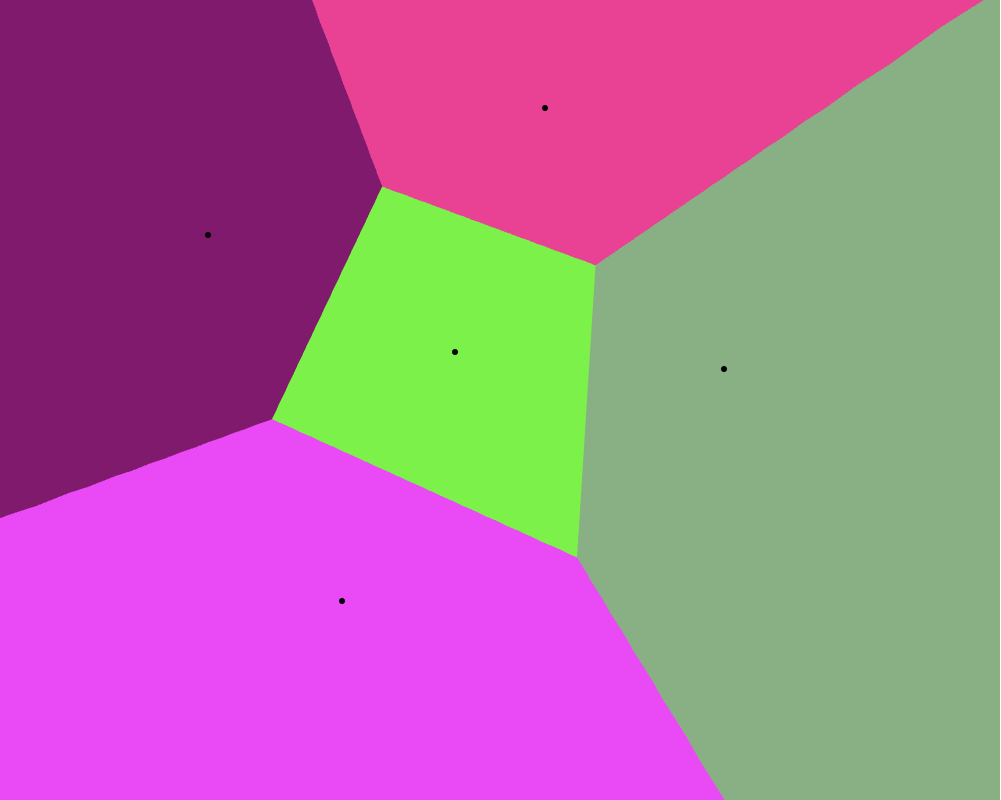
\includegraphics[scale = 0.4]{Диаграмма для задачи}
\end{center}
\section{Формальная постановка задачи}
\subsection{реализовать, исследовать метод}
Даны координаты точек …. Для указанных точек требуется построить диаграмму Вороного, использовуя Алгоритч Форчуна.
\subsection{формат входных данных}
На вход подаются координаты точек, по которым нужно постоить диаграмму Вороного.
\subsection{формат выходных данных}
На выходе должна получиться визуализированная диаграмма Вороного.
\end{document}
